\acfp{FSA} are mathematical abstractions of simple machines. For
example, take a vending machine that will dispense a candy bar when a
quarter has been inserted. There are four actions possible with a
vending machine: insert a quarter, press `coin return' to ask for any
inserted money back, open the window to take the candy bar, and close
the window again. Whether an action is possible (especially the third)
depends on the \emph{state} the machine is in. There are three states:
the begin state, the state where the quarter has been inserted and the
window unlocked (let us call this `ready to dispense'), and the state
where the window is open (which we will call `dispensing').

In certain states, certain
actions are not possible. For instance, in the beginning state the
window can not be opened.

The mathematical description of this vending machine consists of
1.~the list of states, 2.~a table of how the possible actions make the
machine go from one state to another. However, rather than writing
down the table, a graphical representation is usually more insightful.


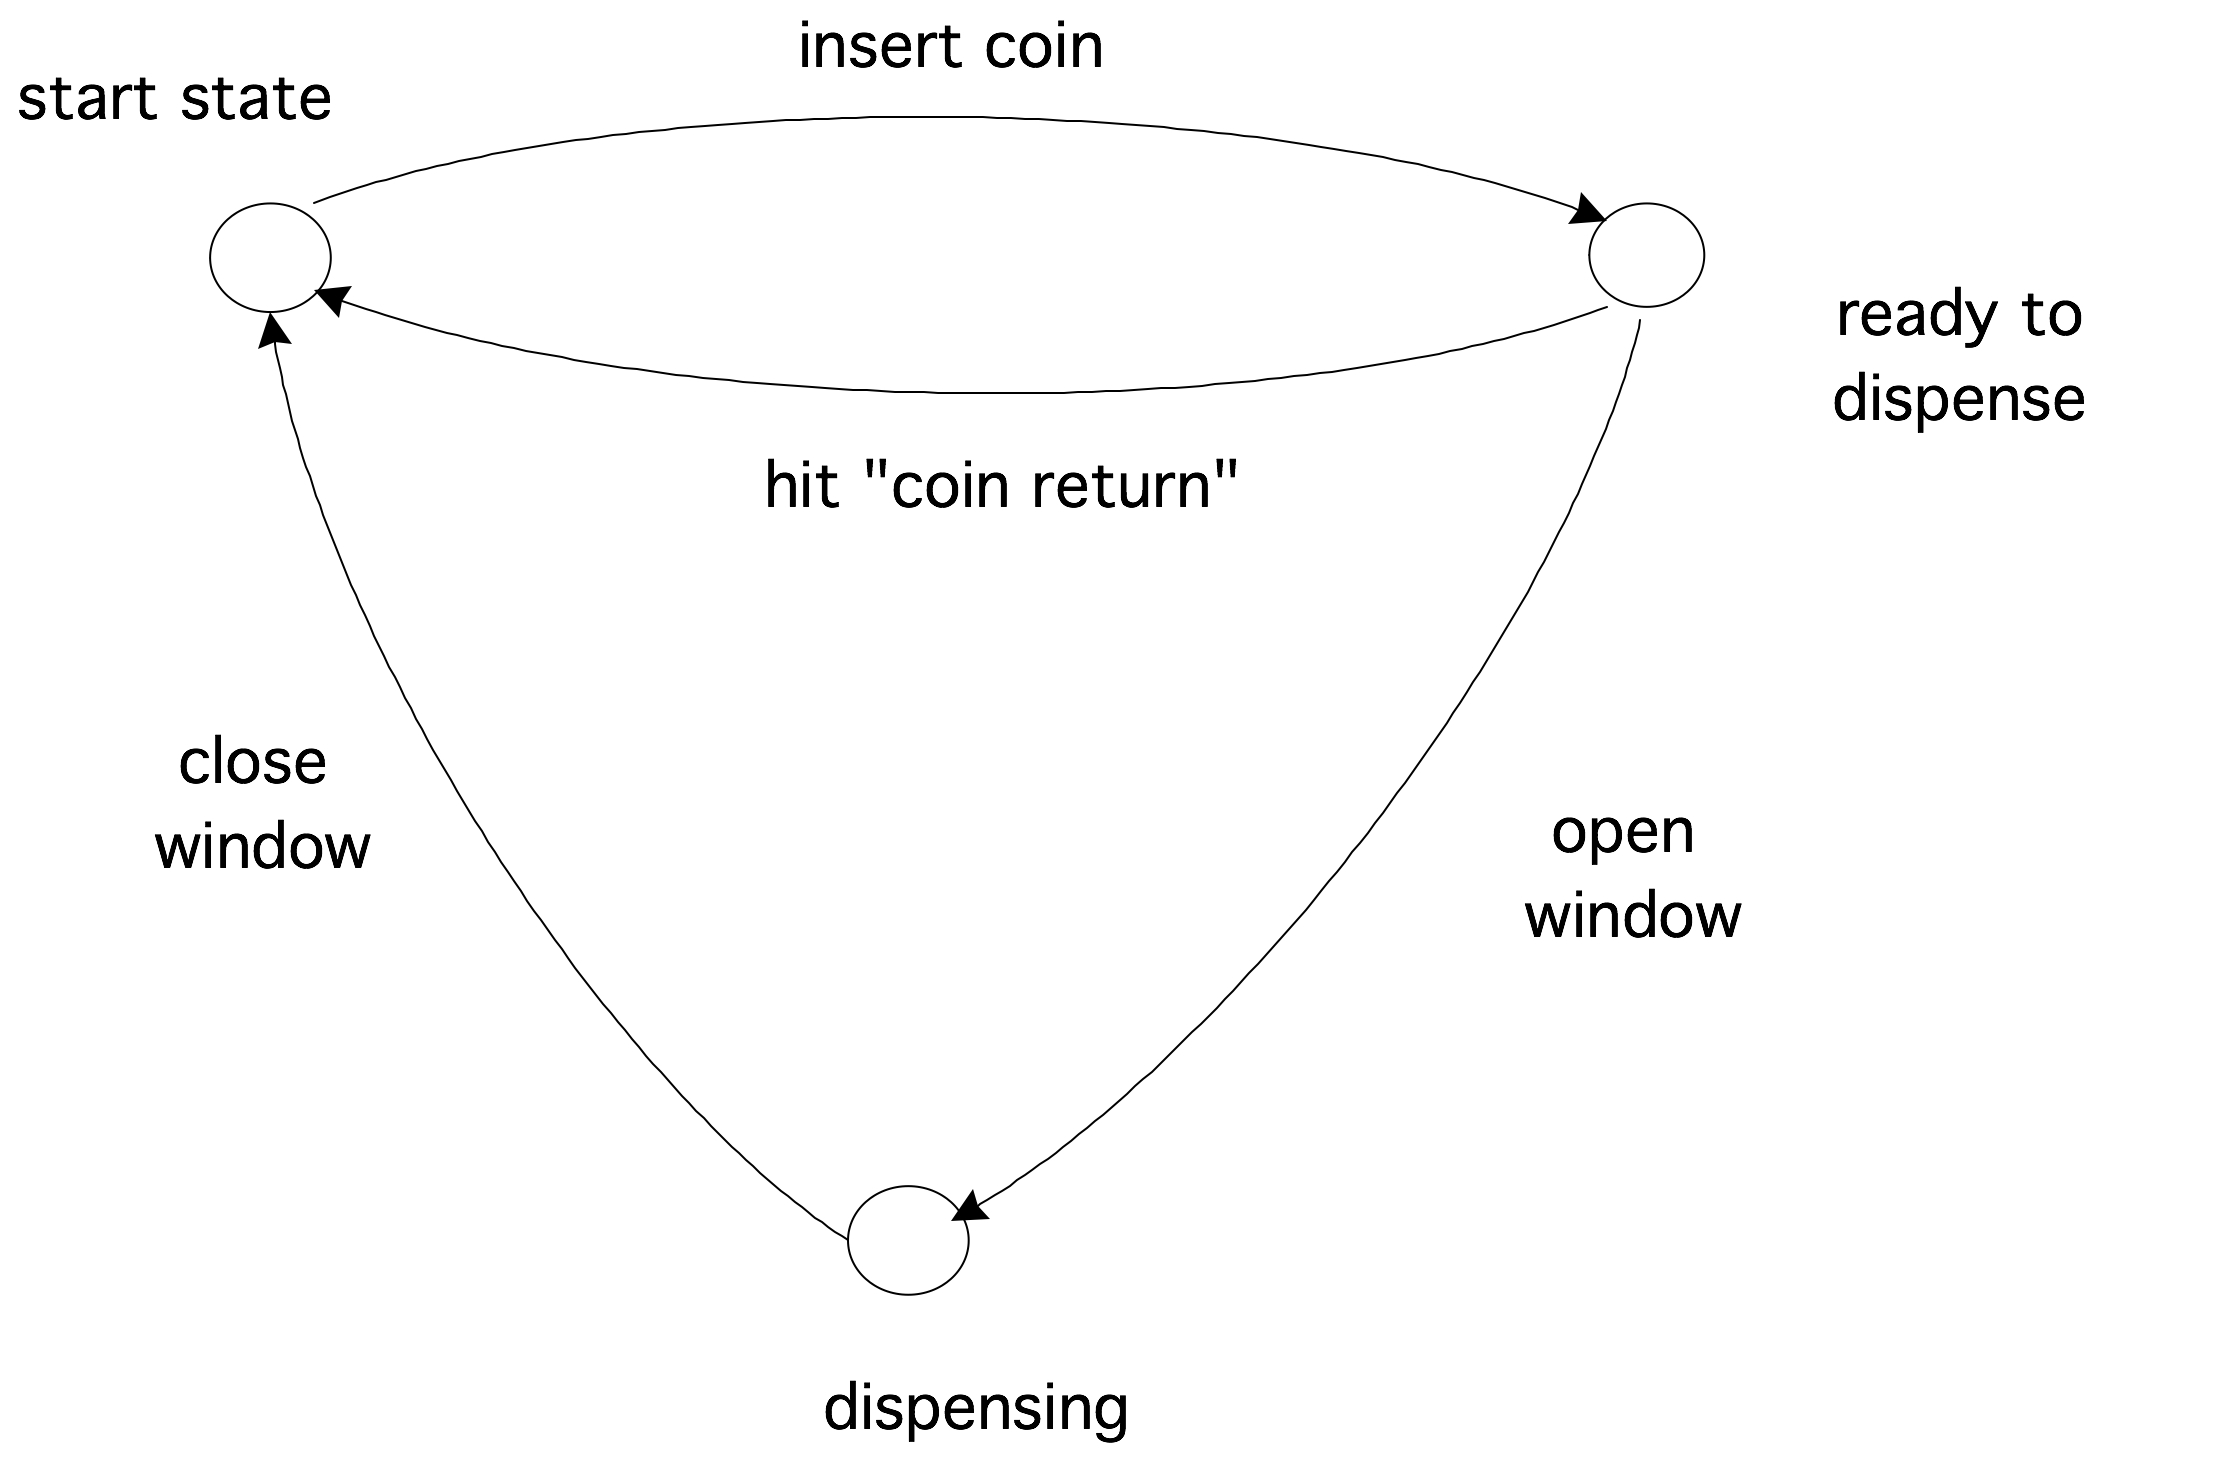
\includegraphics[scale=.15]{graphics-public/fsa}

\endinput

\begingroup\raggedright
\begin{tabular}{p{1.2in}p{1.2in}p{1.2in}p{1.2in}}
  \hfill state:&begin state&accepting&dispensing\\
  action:\\
  insert coin&go to accepting state&go to dispensing state\\
  take candy:&&&go back to begin state
\end{tabular}
\endgroup
